%!TEX root = mb.tex



     
\section{Overview}\label{sec:overview}








In this section, we present \sys's architecture, the threat model and applications supported.


% TO CUT REMOVE: just mentino the figures and no need to explain 
\subsection{System architecture}

\todo{Not quite true -- in APLOMB, we talk about this approach and call it `bounce redirection'. I tried to work it in to the text but it wound up being overly complicated. But if we want to claim that we follow the APLOMB approach, that's still true -- we just need to say we use the bounce approach and why it's less than optimal.}
\sys's system setup is in Fig.~\ref{fig:sys-overview}. This is the same setup as in APLOMB~\cite{aplomb}, 
except for a small difference which we will describe. 
We do not delve into the details, motivation, and gains of APLOMB's setup, and refer the reader to~\cite{aplomb} for details. 
In this setup, there are three parties: enterprise(s), the service provider (SP), and an external site providing
some service. The enterprise runs a gateway (GW) which sends traffic to a middlebox (MB) running in the cloud.
The service provider runs a set of middleboxes. 

There are two typical setups as in Fig.~\ref{fig:sys-overview}.  The first setup, in Fig.~\ref{fig:model1},  occurs when the enteprise communicates with an external site. The second setup occurs when the traffic is sent between two enterprises as in Fig.~\ref{fig:model2}. This allows for a more optimized and faster layout~\cite{aplomb} because  each enterprise has its own gateway.

\sys uses the same setup as APLOMB, except for one modification in the first setup (Fig.~\ref{fig:model1}): in Aplomb, the traffic from SP can go directly to the external site and does not have to go back through the gateway. In \sys, this is unavoidable because the traffic from SP is encrypted and cannot be understood by an external site, unless they have a gateway as in the second setup. However, the setup which is most bandwidth heavy is the second setup, enterprise to enterprise communication where \sys does not change Aplomb's setup.



%The traffic from a client inside the enteprise passes through the gateway on the way out of the enterprise. The gateway redirects this traffic to the middlebox in the cloud.
%After performing various middlebox processing, MB returns the traffic to the gateway. The gateway finally sends the traffic to the external site. 



%Traffic from a client in enterprise 1 passes through the gateway of this enterprise, then it goes  to the middlebox in the cloud, which after processing the traffic, sends it to the gateway of the second enterprise, and the traffic finally arrives at the receiver. This setup allows for better latency, as discussed in~\cite{aplomb}.





\subsection{Threat model}

The goal of \sys is to protect the privacy of the traffic against an attacker at the service provider  
(cloud employee, or hacker gaining access to cloud machines). 
We consider a strong  attacker, one that has gained access to {\em all the data at SP}.
This includes any traffic and communication SP receives from the 
gateway, any old logged information, cloud state, and so on. Nevertheless, we assume that 
SP provides good service and runs middlebox functionality correctly.  We are concerned with 
protecting  the traffic's confidentiality.

We assume that the gateways are trusted, and that they do not leak information.


Some middlebox functionalities (such as intrusion detection or exfiltration detection) have a threat model
of their own regarding the client and the server. For example, intrusion detection assumes that 
the client or the server could misbehave and mount an intrusion attack, but at most one of them misbehaves~\cite{Bro}  
(indeed, if both misbehave, they can send attack traffic to each other encrypted with a shared symmetric key and fundamentally
no one can detect such an attack).  We preserve all these threat models unchanged. These applications rely
on the middlebox to detect attacks in these threat models. Since we assume the middlebox executes
its functions correctly and \sys preserves the functionality of these middleboxes, 
these threat models are irrelevant to the protocols in \sys, and we will not discuss them again. 


\subsection{Goals at gateway}

The goals of NFV and APLOMB are to delegate the burden of managing and configuring
middleboxes (e.g., upgrading, deciding which vendor to use, monitoring), reduce costs of hardware. 
and provide elasticity and fault tolerance; hence \sys should maintain these goals.
%
These translate into a set of requirements for the gateway:
\begin{CompactItemize}
\item Generic functionality: for each {\em type} of middlebox, the gateway should implement a generic functionality, and it should not depend on the specific version and vendor of the software. For example, the gateway should not need to change when a new version of the McAfee firewall is installed, when the admin changes the firewall  from McAfee to Juniper, or when the NAT software gets upgraded. 
\item Should perform lightweight operations.
\item Should not maintain per connection state. The gateway can maintain a small amount of global state, as long as the state does not depend on each connection and does not grow with the packets sent.  \todo{is this contradicted by IDS state at gateway?}
\end{CompactItemize}


\sys achieves these goals, as follows. 

% Firewalls from different vendors may vary significantly in terms of rule syntaxes and organizations. However,
% in general both hardware and software firewalls have a few interfaces. Both ingress and egress of an interface 
% can be associated with an access control list (ACL). Each ACL has a number of rules, possibly in the form 
% <action, protocol, src ip, src port, dst ip, dst port>. Without loss of generality, we take \texttt{pf}, the 
% default firewall under BSD, as an example to illustrate how \sys works with firewalls. Figure \ref{fig:fwrule1} 
% shows an example of \texttt{pf} rules. 

\subsection{\sys overview}


\begin{figure}[t!]
\centering
  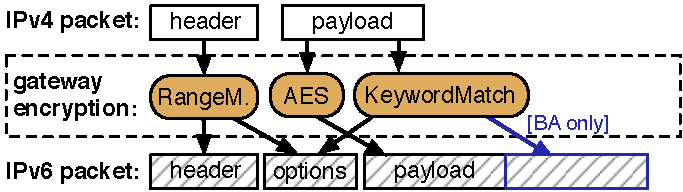
\includegraphics[width=2.0in]{fig/packet.pdf}
\caption{Packet encryption at the gateway. Patterned squares indicate encrypted data. \label{fig:packet}}
\end{figure}





\begin{figure*}[t!]
\centering
  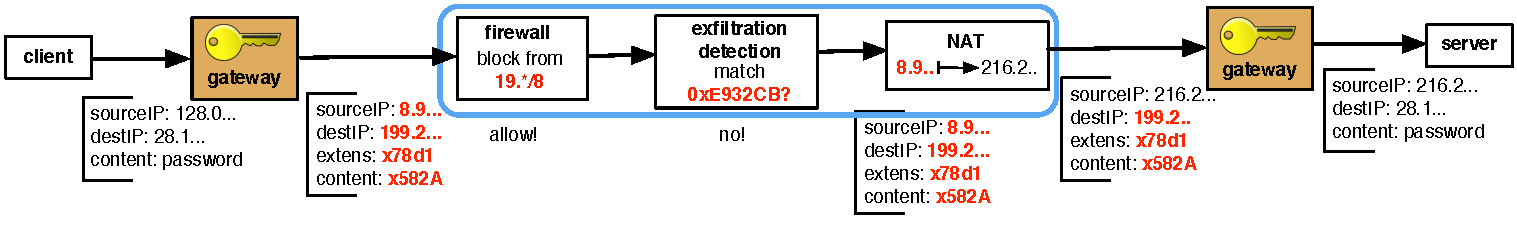
\includegraphics[width=6.7in]{fig/packetpath.pdf}
\caption{Example of packet flow through a few middleboxes. Red indicates encrypted data. \label{fig:packetflow}}
\end{figure*}



To protect privacy of the traffic, \sys encrypts all traffic passing through the middlebox at the cloud. 
As in Fig.~\ref{fig:sys-overview}, the gateway has a secret key $k$; in the setup with two gateways, they share
the same secret key. The gateway encrypts all traffic going to the middlebox in the cloud using \sys's protocols.
The middlebox in the cloud processes {\em encrypted traffic} using \sys's protocols. 
After the processing, the middlebox
will produce encrypted traffic which it sends back to the gateway. The gateway decrypts the traffic using the key $k$.

Throughout this process, middleboxes at SP handle only encrypted traffic and never get the decryption key. This ensures
that an attacker that steals all data from SP, will only see encrypted traffic and hence protects the privacy of the 
traffic. 
\sys encrypts IP addresses, ports, and the payload of the packet, thus protecting the privacy of all these parameters. 
%Middleboxes at the cloud operate over the encrypted values in each packet, and do not have access to the decrypted data.

\sys enables encrypted operation for {\em all} typical middleboxes in outsourcing scenarios, despite substantial differences in how the middleboxes operate, what packet data they access, and whether they modify or merely observe packets.
  We classify middleboxes in  two broad categories based on the type of data they access: {\em header-only} middleboxes and {\em bytestream-aware} middleboxes.
  Some middleboxes are `header-only' middleboxes: they operate over packet headers (\eg{}, IP, TCP, or even HTTP headers) on a packet-by-packet basis.
Examples  include IP Firewalls and Network Address Translators (NATs).

\todo{not sure it is clear that bytestream-aware are more expensive; also what is the work of the gateway for the bytestream ones?}

  Other middleboxes are `bytestream-aware.' These middleboxes operate over a TCP bytestream -- the concatenation of all {\it payloads} -- and hence must keep substantial state per connection.
  For example, many Intrusion Detection Systems (IDS) are bytestream-aware; in order to detect attack signatures that span across multiple packets they keep a buffer which with copies of each payload it has forwarded.
  It uses these payloads to to reconstruct the TCP bytestream, just as the client will observe at the application layer; the IDS can then scan this bytestream for malicious substrings.
  Web proxies are also bytestream-aware; rather than keeping a copy of packets the proxy forwards, the proxy performs {\it session termination}. 
  When a client opens a new HTTP connection, a typical proxy will capture the client's SYN packet and open a new connection to the client, as if it were the web server the client wished to connect to. 
  The proxy also maintains second connection in the background to the original web server, as if it were the client. 
  Session termination allows the proxy to cache entire images (which usually span multiple packets) and respond to client requests with cached data as if it were the server.
  In Table~\ref{tab:apps-ops}, we list each middlebox, the cryptographic tools used to encrypt it, and whether it is a bytestream-aware (BA) or header-only (HO) middlebox.

  As we will see, to support header-only middleboxes, the \sys gateway can also operate in a header-only fashion, encrypting each header field (\eg{}, IP address, port number) independently.
  However, to support bytestream-aware appliances, the \sys gateway also needs to be be bytestream aware, in order to encrypt the concatenation packet payloads.
  The one exception to this rule -- that header-only middleboxes can be served by a header-only gateway, while bytestream-aware middleboxes require a bytestream-aware gateway -- is web proxying.
  Proxies are bytestream-aware, but can be served by a header-only middlebox when they do not allow pipelined requests.
  As we will discuss in \S\ref{sec:proxies}, the gateway can encrypt the HTTP header values on a packet-by-backet basis without requiring any TCP bytestream reconstruction so long as HTTP pipelining is not enabled. 


To understand \sys, Fig.~\ref{fig:packetflow} shows the end-to-end flow of a packet through three middleboxes in the cloud. The traffic on the path gateway-SP-gateway is IPv6, a requirement of our RangeMatch scheme. If the traffic into the gateway is IPv4, the gateway converts it to IPv6, using \todo{Example}. The first step in Fig.~\ref{fig:packetflow} is that the gateway encrypts the packet. As shown in Fig.~\ref{fig:packet}, the header information such as IP addresses and ports gets encrypted with RangeMatch and placed into the header and the extension field of the encrypted packet. The payload gets encrypted using the KeywordMatch scheme, and some auxiliary encrypted information is also placed in the extension field. Back to Fig.~\ref{fig:packetflow}, the packet passes through the firewall which tries to match the encrypted information from the header against  encrypted rules, and decides to allow the packet. Next, the exfiltration device checks for any suspicious (encrypted) strings on the packet payload, and not finding any, it allows the packet  to continue to the NAT. The NAT maps the source IP address to an external IP address. Back at the gateway, the gateway decrypts the packet. 

Independent of \sys, the gateway (G) can use SSL on the links client-G,  G-server, G-SP and SP-G. 





